%!TEX root = ../main.tex

\section{Tree-Like Unraveling}\label{sec:unraveling}
We next describe a notion of \emph{tree unravelings} for $\FGF$.
A ``truncated'' form of these unravellings will be employed afterwards in the construction of the companion structures required for~\cref{thm:main-technical-thm}.
The truncation is necessary to keep the resulting structure finite, as tree unravellings of structures containing cycles are infinite.
This is similar to the approach taken by Otto to construct the finite companions for the van Benthem charactisation of modal logic with universal modalities~\cite[Proof of Lemma 38]{Otto04}.
Our approach is similar to the construction of finite companions in the van Benthem Characterisation of modal logic with the universal modality by Otto~\cite[Proof of Lemma 38]{Otto04}.
However, novel ideas are required to make this construction applicable to the case of higher-arity relations.

For structures $\str{A}$ with a distinguished binary predicate $\relNext^{\str{A}}$, we employ a tailored terminology from graph theory, as expected.
For instance, whenever $(\eleme_1, \eleme_2) \in \relNext^{\str{A}}$, we call the element $\eleme_2$ a \emph{child} of $\eleme_1$. Respectively, we call $\eleme_1$ a \emph{parent} of $\eleme_2$.
A \emph{root} is an element without parents.
The set of \emph{descendants} of an element $\eleme$ is the smallest set containing $\eleme$ that is closed under taking children (\ie{} if an element is in the set then so are its children).
We call a structure $\str{A}$ a \emph{forest} if every element has at most one parent and is a descendant of some root.
A model is a tree model if it is a forest and has exactly one root.
It is well-known that with a suitable notion of unraveling~\cite[Prop. 3]{Rosen97} one can show that every satisfiable modal logic formula has a tree model.

Our goal is to design a notion of unravelling for $\FGF$ satisfying the following theorem:
\begin{restatable}{theorem}{thminfunraveling}\label{thm:inf-unraveling-upgrading}
  Let $\str{A}, \elemtuplea \bisimto_{\FGF} \str{B}, \elemtupleb$ for two pointed structures.
  Then there are tree models $\unravel{A}, \elemtuptuplea$ and $\unravel{B}, \elemtuptupleb$ which are both:
  \begin{itemize}
    \item $\FGF$-similar to the original structures: $\unravel{A}, \elemtuptuplea \bisimto_{\FGF} \str{A}, \elemtuplea$ and $\unravel{B}, \elemtuptupleb \bisimto_{\FGF} \str{B}, \elemtupleb$
    \item $\GF$-bisimilar: $\unravel{A}, \elemtuptuplea \bisimto_{\GF} \unravel{B}, \elemtuptupleb$.
  \end{itemize}
\end{restatable}

\noindent
The \emph{HAF}-unravelling~\cite[Sec 3.3]{Bednarczyk21} introduced by Bednarczyk produces a tree model which is \FGF-bisimilar to a given \FGF-model, but unfortunately fails to satisfy the above theorem.
Consider the two finite structures depicted in \cref{fig:unravel-haf}.
Both of them are identical to their HAF-unravelling as they are already HAFs.
Yet, they can be distinguished by a $\GF$ sentence $\exists{x,y}. \relE(x,y) \land \lnot (\exists z. \relP(x,y,z))$.
Since both structures are $\FGF$ bisimilar, this shows that HAF-unravellings do not satisfy \cref{thm:inf-unraveling-upgrading} even in the finite case.

\begin{figure}[H]
  \centering
    \begin{tikzpicture}[baseline=(current bounding box.north)]
        \draw[tolbrightGreen, line cap=round, line width=2em] (-0em,8em) -- ++(0,-8em);
        \draw[tolbrightYellow, line cap=round, line width=0.5em, -{Latex[length=2em]}] (0,4em) -- (0,0em);

        \draw [black, line width=0.1em, fill=white] (0em, 8em) circle [radius=0.8em] node[anchor=center] {1};
        \draw [black, line width=0.1em, fill=white] (0em, 4em) circle [radius=0.8em] node[anchor=center] {2};
        \draw [black, line width=0.1em, fill=white] (0em, 0em) circle [radius=0.8em] node[anchor=center] {3};

        \begin{scope}[xshift=10em]
            \draw[tolbrightGreen, line cap=round, line width=2em] (-0em,8em) -- ++(0,-8em);
            \draw[tolbrightYellow, line cap=round, line width=0.5em, -{Latex[length=2em]}] (0em,4em) -> (6em,2em);
            \draw[tolbrightYellow, line cap=round, line width=0.5em, -{Latex[length=2em]}] (0,4em) -- (0,0em);

            \draw [black, line width=0.1em, fill=white] (0em, 8em) circle [radius=0.8em] node[anchor=center] {1};
            \draw [black, line width=0.1em, fill=white] (0em, 4em) circle [radius=0.8em] node[anchor=center] {2};
            \draw [black, line width=0.1em, fill=white] (0em, 0em) circle [radius=0.8em] node[anchor=center] {3};
            \draw [black, line width=0.1em, fill=white] (6em, 2em) circle [radius=0.8em] node[anchor=center] {3'};

            \node[tolbrightGreen] at (-2em, 6em) {P};
            \node[tolbrightYellow] at (-1.5em, 2em) {E};
            \node[tolbrightYellow] at (3em, 4em) {E};
        \end{scope}

        \node[font=\Large] at (5em, 4em) {$\sim_{FGF}$};

        \node[tolbrightGreen] at (-2em, 6em) {P};
        \node[tolbrightYellow] at (-1.5em, 2em) {E};
    \end{tikzpicture}%
    \caption{Two FGF-bisimilar HAFs which are not GF-bisimilar. Relations are drawn top to bottom, so the green area marks the relation $\relP(1,2,3)$}%
    \label{fig:unravel-haf}
\end{figure}

We next describe a new notion of unraveling for $\FGF$ which, as we see later, satisfies \cref{thm:inf-unraveling-upgrading}.
This unraveling is closely related to the $\FGF$-game, with elements that correspond to sequences of moves in this game.
We begin with a description of the domain of the unraveling.

\noindent \textbf{Domain of the unraveling}
Let $\str{A}, \elemtuplea^{(0)}$ be a pointed structure where $\elemtuplea^{(0)}$ is just tuple of elements from $A$, labelled with a zero index as it is the starting tuple for the unraveling.
We define a \emph{bisimulation sequence} as a sequence of moves that Spoiler takes in one of the possible plays of the $\FGF$-bisimulation game involving this structure, excluding moves where Spoiler picks an empty infix.
Formally, an $\ell$-\emph{bisimulation sequence} is a word in $A^*{(\N\N{}A^{*})}^{\ell}$, represented by a sequence of the form $\elemtuplea^{(0)}(i^{(1)}, j^{(1)})\elemtuplea^{(1)}\cdots(i^{(\ell)}, j^{(\ell)})\elemtuplea^{(\ell)}$, where each $a^{(k)}$ is a live tuple from $\str{A}$ and $i^{(k)}, j^{(k)}$ are indices with $i < j$ for which $\elemtupleafromto{i^{(k)}}{j^{(k)}}^{(k-1)} = \elemtupleafromto{1}{j^{(k)}-i^{(k)}+1}^{k}$.
Bisimulation sequences are denoted by greek letters $\rho, \sigma, \theta, \ldots$ and for
a bisimulation sequence $\sigma$ we refer to the parameter $\ell$ in the above definition as the \emph{level} of $\sigma$.
We say that a sequence $\theta$ \emph{extends} a sequence $\rho$ is $\rho$ is a prefix of $\theta$.
Intuitively, the set $\Seq{A}$ of all bisimulation sequences for a structure $\str{A}$ collects all possible ways in which Spoiler can explore this structure.
For any $\ell$-bisimulation sequence, if $\str{B}, \elemtupleb^{(0)}$ is a structure that is \FGF-bisimilar to $\str{A}, \elemtuplea^{(0)}$, then we can apply~\ref{bisim:fforth} $\ell$ times to find tuples $\elemtupleb^{1}, \ldots, \elemtupleb^{\ell}$ for a corresponding bisimulation sequence in $\str{B}$.
These represent the moves of Duplicator in the game.
Below are some examples of bisimulation sequences:
\begin{figure}[H]
  \centering
    \begin{minipage}[t]{0.2\textwidth}
        \raggedleft%
        \vspace{0pt}
        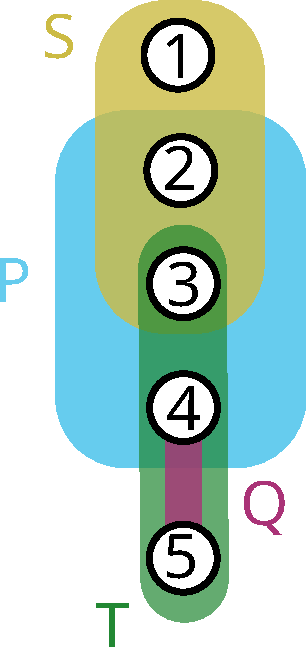
\includegraphics[scale=0.5]{res/example-struct-1}
    \end{minipage}
    \hspace{4em}
    \begin{minipage}[t]{0.6\textwidth}
      {%
      \newcommand{\tups}{{\color{tolbrightYellowDarker}\elemtuples}}%
      \newcommand{\tupp}{{\color{tolbrightCyanDarker}\elemtuplep}}%
      \newcommand{\tupt}{{\color{tolbrightGreen}\elemtuplet}}%
      \newcommand{\tupq}{{\color{tolbrightPurple}\elemtupleq}}%
      The picture on the left shows a structure with the relations: $(1,2,3) \in \relS^{\str{A}}$, $(2,3,4) \in \relP^{\str{A}}$, $(3,4,5) \in \relT^{\str{A}}$, $(4,5) \in \relQ^{\str{A}}$.

      \vspace{1ex}
      Let $\tups = (1, 2, 3), \tupp = (2, 3, 4), \tupt = (3, 4, 5), \tupq = (4,5)$.

      \vspace{1ex}
      Some examples of bisimulation sequences in this structure are:
      \begin{itemize}
          \item $\tups(3,3)\tupt$,
          \item $\tups(2,3)\tupp(2,3)\tupt$.
      \end{itemize}

      Bisimulation sequences are not required to use maximal infixes, so the following are also valid bisimulation sequences:
      \begin{itemize}
          \item $\tups(2,2)\tupp$,
          \item $\tups(3,3)\tupt(2,2)\tupq$.
      \end{itemize}
      }
    \end{minipage}
    \caption{Examples of bisimulation sequences.}%
    \label{fig:bisim-seq-examples}
\end{figure}

Let $\Seq{\str{A}}$ be the set of all bisimulation sequences for a structure $\str{A}$.
There is a natural projection from a bisimulation sequence $\sigma \in \Seq{A}$ to tuples of $\str{A}$: for $\sigma = \cdots (i,j) \elemtuples$, we define the projection $\Pi(\sigma)$ as $\Pi(\sigma) = \elemtuples$.
Intuitively, this projection gives the tuple of selected elements in the bisimulation game after playing the moves of $\sigma$.

To construct the domain of the unraveling, we combine bisimulation sequences with natural numbers.
This allows us to define a projection that maps to individual elements of $\str{A}$, instead of tuples.
A \emph{tagged bisimulation sequence} of a structure $\str{A}$ is a tuple $(\sigma, k) \in \Seq{A} \times \mathbb{N}$ such that
\begin{itemize}
  \item $\sigma = \elemtuplea$, $k \ge 1$ and $k \le |\elemtuplea|$ for some $\elemtuplea \sqin A$, or
  \item $\sigma = \cdots (i,j) \elemtuplea$, $k \ge (j-i+1) + 1$ and $k \le |\elemtuplea|$ for some $\elemtuplea \sqin A$.
\end{itemize}
For more background on these conditions, see \cref{ex:tagged-bisim-seq}.
The \emph{domain of the unraveling} for a structure $\str{A}$, denoted by $\unraveldom{A}$, is the set of all tagged bisimulation sequences of the structure $\str{A}$.
For a tagged bisimulation sequence $e \in \unraveldom{A}$ that can be decomposed as $e = (\rho, k)$, we use the notation $\seq{e} = \rho$ and $\ctr{e} = k$ to denote the sequence and the counter of this tagged bisimulation sequence, respectively.
Since the counter is an index into the components of $\Pi(\seq{e})$, we can define the projection $\pi(e)$ from tagged bisimulation sequences to elements of $A$ as: $\pi(e) = \Pi(\seq{e})_{\ctr{e}} = \elema_{\ctr{e}}$ for $\seq{e} = \cdots\elemtuplea$.
\begin{example}\label{ex:tagged-bisim-seq}
   {%
     \newcommand{\tups}{{\color{tolbrightYellowDarker}\elemtuples}}%
     \newcommand{\tupt}{{\color{tolbrightGreen}\elemtuplet}}%
     \newcommand{\es}{{\color{tolbrightYellowDarker}s}}%
     \newcommand{\et}{{\color{tolbrightGreen}t}}%
     Consider the bisimulation sequences from \cref{fig:bisim-seq-examples}.
     The tagged bisimulation sequences for the level-0 bisimulation sequence $\sigma$ with $\sigma = \tups$ are: $a = (\sigma, 1)$, $b = (\sigma, 2)$ and $c = (\sigma, 3)$.
     These project to the components of the tuple $\tups$: $\pi(a) = \es_{1} = 1$, $\pi(b) = \es_{2} = 2$ and $\pi(c) = \es_{3} = 3$.
     Now consider the bisimulation sequence $\rho$ with $\rho = \tups(3,3)\tupt$.
     Recalling the bisimulation game, this sequence represents the move from $\tups$ to $\tupt$, sharing the element ``3''.
     There are tagged bisimulation sequences $d = (\rho, 2)$ and $e = (\rho, 3)$ which project to the domain elements ``4'' and ``5''.
     However, there is no tagged bisimulation sequence for the sequence $\rho$ that projects to ``3''.
     While $(\rho, 1)$ projects to ``3'' according to the definition of $\pi$, it is not a tagged bisimulation sequence as it violates the ``$k \ge (j-i+1) + 1$'' condition in the above definition.
     Note that $c = (\sigma, 3)$ projects to ``3'', so there already is a tagged bisimulation sequence that projects to ``3'', using the sequence $\sigma$.
     Intuitively, the condition ensures that for the move from a tuple $\tups$ to a tuple $\tupt$ in the game, there is at most one tagged bisimulation sequence projecting to each shared element.
     Stated differently, tagged bisimulation sequences correspond one-to-one to unshared elements of moves in the bisimulation game.
   }
\end{example}

On the domain of the unraveling, the binary relation $\relNext \subseteq \unraveldom{A} \times \unraveldom{A}$ is defined such that $(s, t) \in \relNext$ if either:
\begin{description}
  \item[\desclabel{(addCtr)}{next:addctr}] $s = (\sigma, k)$ and $t = (\sigma, k + 1)$ for some $\sigma \in \Seq{A}$ and $k \in \N$, or
  \item[\desclabel{(addSeq)}{next:addseq}] $s = (\sigma, j)$ and $t = (\sigma(i,j)\elemtuplea, (j-i+1) + 1)$ for some $\sigma \in \Seq{A}$, $\elemtuplea \sqin A$ and $i,j \in \N$.
\end{description}
The picture below shows an example for this definition.
It depicts a subset of the domain of the unraveling of the structure $\str{E}$ (taken from \cref{fig:unravel-haf}) and the $\relNext$ relation on this domain.

\begin{figure}[H]
  \centering
  {
\newcommand{\tupp}{{\color{tolbrightGreenDarker}\elemtuplep}}%
\newcommand{\tupe}{{\color{tolbrightYellowDarker}\elemtuplee}}%

\begin{tikzpicture}
  \draw[tolbrightGreen, line cap=round, line width=2em] (-0em,8em) -- ++(0,-8em);
  \draw[tolbrightYellow, line cap=round, line width=0.5em, -{Latex[length=2em]}] (0,4em) -- (0,0em);

  \draw [black, line width=0.1em, fill=white] (0em, 8em) circle [radius=0.8em] node[anchor=center] {1};
  \draw [black, line width=0.1em, fill=white] (0em, 4em) circle [radius=0.8em] node[anchor=center] {2};
  \draw [black, line width=0.1em, fill=white] (0em, 0em) circle [radius=0.8em] node[anchor=center] {3};

  \node[anchor=base] at (0em,-4em) {{\Huge $\str{E}$}};
  \node at (3.5em, 4em) { {\Huge $\leadsto$} };

  \node[anchor=south west] at (4em, 10em) { $\tupp = (1,2,3)$ and $\tupe = (2,3)$ };

  \begin{scope}[xshift=7em, yshift=8em]
    \tikzset{element/.style = {
        inner sep=0.25em, fill=white, rounded corners=0.7em, draw=black
      }};
    \tikzset{edge from parent/.style = {draw,->}};
    \node[element] (p1) {$(\tupp, 1)$}
      [level distance=4em, grow=down, sibling distance=7em]
      child[missing]
      child[grow=down] { node[element] (p2) {$(\tupp, 2)$}
        child [missing]
        child [grow=down] { node[element] (p3) {$(\tupp, 3)$}
        }
        child [] { node[element] (p22e2) {$(\tupp(2,2)\tupe, 2)$} }
      }
      child { node[element] (p11p2) {$(\tupp(1,1)\tupe, 2)$}
        child [missing]
        child [missing]
        child { node[element] (p11p3) {$(\tupp(1,1)\tupp, 3)$} }
      }
    ;

    \node[anchor=center] (d2) at ($(p3.east)!0.5!(p22e2.west)$) { \ldots };
    \node[anchor=center] (dside) at (13em, -5em) { \ldots };

    \draw[-{Straight Barb[]}, loosely dotted, thick] (p2) -- (d2);
    \draw[-{Straight Barb[]}, loosely dotted, thick] (p11p2) -- (dside);

    \node[text width=15em, align=left, anchor=base west] at (0em,-12em) {{\hspace{2em}\huge$\unraveldom{E}$} \\ (domain of the unraveling)};

    \node[text width=25em, align=left, anchor=south west] at (12em, -3em) {
      \small
      $((\tupp, 1), (\tupp, 2)) \in \relNext$ by~\ref{next:addctr}

      \vspace{1ex}
      $((\tupp, 2), (\tupp(2,2)\tupe, 2)) \in \relNext$ by~\ref{next:addseq}

      \vspace{1ex}
      $((\tupp, 1), (\tupp(1,1)\tupp, 3)) \notin \relNext$ by~\ref{next:addseq} eq. 1

      \vspace{1ex}
      $((\tupp, 2), (\tupp(1,1)\tupp, 3)) \notin \relNext$ by~\ref{next:addseq} eq. 2
    };
  \end{scope}

\end{tikzpicture}
}

\end{figure}

\noindent{%
\newcommand{\tupp}{{\color{tolbrightGreenDarker}\elemtuplep}}%
\newcommand{\tupe}{{\color{tolbrightYellowDarker}\elemtuplee}}%
The relation $\relNext$ links elements which represent consecutive components within a tuple of the base structure, but following the structure imposed by the bisimulation sequences, as explained below.
There are two cases.
In the~\ref{next:addctr} case we keep the bisimulation sequence the same and increase the counter by one.
This case is represented by vertical arrows in the above picture.
For example, the elements $(\tupp, 1)$ and $(\tupp, 2)$ represent the elements $1$ and~$2$ which are consecutive elements of the tuple $\tupp$, so $((\tupp, 1), (\tupp, 2)) \in \relNext$.
In the~\ref{next:addseq} case, we extend the bisimulation sequence with one more bisimulation move.
This case is represented by arrows that branch sideways in the above picture.
Extending the sequence is only allowed if we start from the element that represents the last (with the highest counter) shared element and end at the first (with the lowest counter) unshared element.
As an example, consider the element $(\tupp, 2)$.
The bisimulation sequence $\tupp(2,2)\tupe$ represents the move from $\tupp$ to $\tupe$, while keeping the second element of $\tupp$ fixed.
Thus, the last shared element is $(\tupp, 2)$ and the first unshared element is $(\tupp(2,2)\tupe, 2)$, so those two elements are in $\relNext$.
Consider now the element $(\tupp(1,1)\tupp, 3)$.
Its bisimulation sequence $\tupp(1,1)\tupp$ is also an extension of the bisimulation sequence of $(\tupp, 2)$.
However, it represents a move from $\tupp$ to $\tupp$ sharing only the first element.
The last (and only) shared element in this move is $(\tupp, 1)$, so there is no edge from $(\tupp, 2)$ to $(\tupp(1,1)\tupp, 3)$.
Similarly, there is no edge from $(\tupp, 1)$ to $(\tupp(1,1)\tupp, 3)$, as $(\tupp(1,1)\tupp, 3)$ is not the first unshared element.
}

We show that the relation $\relNext$ forms a forest:
\begin{lemma}
  For a structure $\str{A}$, the domain of the unraveling $\unraveldom{A}$ together with the relation $\relNext$ is a forest. The roots are the elements composed of a 0-bisimulation sequence and a counter equal to 1.
\end{lemma}
\begin{proofsketch}
  The counter of an element $t \in \unraveldom{A}$ is \emph{minimal} if the counter is the smallest among elements of the domain with the same bisimulation sequence as $t$.
  The key observation now is that if $(s,t) \in \relNext$ because of case~\ref{next:addseq}, then the counter of $t$ is minimal, while if $(s,t) \in \relNext$ because of case~\ref{next:addctr}, then the counter of $t$ cannot be minimal (since $s$ is witness that there are elements with a smaller counter).
  Take an element $t \in \unraveldom{A}$ with $(s, t) \in \relNext$ for some element $s \in \unraveldom{A}$.
  If the counter is not minimal, then the unique parent $s$ is element obtained by decreasing the counter by one.
  If the counter is minimal and cannot be further decreased, then the unique parent $s$ is the element with the sequence reduced by one move and counter equal to the index $j$ as specified in the~\ref{next:addseq} case of the definition of $\relNext$.
  We observe that the parent of an element either has a sequence with a decreased level or it has a sequence with the same level but a decreased counter.
  Thus, taking parents repeatedly must end in a root at some point.
  Therefore every element is a descendant of some root and has at most one parent, proving that $\relNext$ forms a forest.
  The only elements without a parent are those composed of a 0-bisimulation sequence and a minimal counter.
  Since $(\sigma, 1) \in \unraveldom{A}$ for any 0-bisimulation sequence $\sigma \in \Seq{A}$, the roots are exactly the elements composed of a 0-bisimulation sequence and a counter equal to 1.
\end{proofsketch}

Finally, we formalize the property that $\relNext$ links elements that map to consecutive elements in the base structure:
\begin{lemma}\label{lem:projection-next}
For elements $s, t \in \unraveldom{A}$ with $\ctr{t} \ge 2$ and $(s,t) \in \relNext$, if $\elemtuplea \sqin \unraveldom{A}$ is the tuple such that $\seq{t} = \cdots \elemtuplea$, then $\pi(s) = a_{k-1}$ and $\pi(t) = a_{k}$ for $k = \ctr{t}$.
\end{lemma}
\begin{proofsketch}
  Let $\seq{s} = \cdots \elemtupleb$.
  Since $(s,t) \in \relNext$, the bisimulation sequence $\seq{t}$ extends $\seq{s}$.
  Thus, $\elemtupleb$ and $\elemtuplea$ must an share an infix (by definition of bisimulation sequences).
  The definition of $\relNext$ restricts the counters $\ctr{s}$ and $\ctr{t}$ such that the equality $b_{\ctr{s}} = a_{\ctr{t}-1}$ holds, implying the property of the lemma.
\end{proofsketch}
\begin{proof}
  Note that $\pi(t) = a_{\ctr{t}} = a_{k}$ by definition of the projection $\pi$.
  We prove that $\pi(s) = a_{k-1}$ by case analysis on the two cases of $\relNext$.
  The~\ref{next:addctr} case is simple: in this case $\seq{s} = \seq{t}$ and $\ctr{s} = k - 1$, so the property follows directly from the definition of $\pi$.
  For the~\ref{next:addseq} case, let $\seq{t} = \seq{s} (i,j) \elemtuplea$ and $\seq{s} = \cdots \elemtupleb$.
  Further, in this case $k = (j - i + 1) + 1$ and $\ctr{s} = j$.
  By the fact that $\seq{t}$ is a bisimulation sequence, we know that $\elemtupleafromto{1}{j-i+1} = \elemtuplebfromto{i}{j}$.
  In particular, it follows that $\pi(s) = b_{j} = a_{j-i+1} = a_{k-1}$, concluding the proof.
\end{proof}

\noindent
\textbf{Relations in the unraveling}
A tuple of elements $(e_{1}, \ldots, e_{n})$ is a \emph{next-chain} if consecutive elements are related by $\relNext$, namely $(e_{i}, e_{i+1}) \in \relNext$ for all $i < n$.
If the length $n$ of the next-chain is less than $\ctr{e_{n}}$, then we know by \cref{lem:projection-next} that the projection of the chain is $\elemtuplee_{(\ctr{e_{n}}-n+1)\ldots{}\ctr{e_{n}}}$, where $\elemtuples$ is the last tuple of $\seq{e_{n}}$.
We define the tree unraveling such that relations are only realized by tuples which are next-chains.
Additionally, we limit the length of the chain to be less than the counter of the last element of the tuple.
For any tuple $\elemtuptupler$ from the domain of the unraveling, define the \emph{bound} of $\elemtuptupler$ (denoted by $\bound{\elemtuptupler}$) to be equal to the counter of its last element.
Formally, $\bound{\elemtuptupler} = \ctr{r_{|\elemtuptupler|}}$.
Let $\str{A}, \elemtuplea$ be a structure and $\unraveldom{A}$ be the domain of the unraveling.
Let $\elemtuptuplea = ((\elemtuplea, 1), \ldots, (\elemtuplea, |\elemtuplea|))$.
The \emph{tree unraveling} $\unravel{A}, \elemtuptuplea$ is the tree with root $(\elemtuplea, 1)$ and all descendants according to the relation $\relNext$.
For relations $\relR \in \Sigma$, we let $\elemtuptupler \in \relR^{\unravel{A}}$ if and only if:\begin{enumerate}
  \item $\pi[\elemtuptupler] \in \relR^{\str{A}}$,
  \item $\bigwedge_{k=1}^{|\elemtuptupler|-1}{(\elemr_{k},\elemr_{k+1}) \in \relNext}$, and
  \item $|\elemtuptupler| \le \bound{\elemtuptupler}$
\end{enumerate}
The second and third condition restrict live tuples to be next-chains with a length bounded by the counter of the last element of the tuple, as discussed before.

We illustrate the construction with an example.
The picure below shows the tree unraveling $\unravel{E}$ of the structure $\str{E}$ from the previous example with root $(\elemtuplep, 1)$, where again $\elemtuplep = (1,2,3)$ and $\elemtuplee = (2,3)$.
\begin{figure}[H]
  \centering
  \begin{tikzpicture}
  \tikzset{element/.style = {inner sep=0.25em, fill=white, solid, rounded corners=0.7em, draw=black}};
  \tikzset{edge from parent/.style = {draw, thick}};

  \begin{scope}[xshift=-14em, yshift=2.5em]
    \draw[tolbrightGreen, line width=0.4em, -{Stealth[round]}] (0,0) -- +(3em, 0) node[anchor=west] { $P$ };
    \draw[tolbrightYellow, line width=0.25em, -{Stealth[round]}] (0,-1.5em) -- +(3em, 0) node[anchor=west] { $E$ };
    \draw[black, thick] (0,-3em) -- +(3em, 0) node[anchor=west] { $\relNext$ };
  \end{scope}

  \node[element] (p1) {$(\elemtuplep, 1)$}
    [level distance=5em]
    child[grow=220, every child node/.style={anchor=east}] {
      node[element] (p2) {$(\elemtuplep, 2)$} edge from parent [draw=none]
      %
      child[grow=190]  {node[element]              (p12p3) {$(\elemtuplep(1,2)\elemtuplep, 3)$}}
      child[grow=240]  {node[element]              (p22e2) {$(\elemtuplep(2,2)\elemtuplee, 2)$}}
      child[grow=down] {node[element,anchor=north] (p3)    {$(\elemtuplep, 3)$}}
    }
    child[grow=-50, every child node/.style={anchor=west}] {
      node[element] (p11p2) {$(\elemtuplep(1,1)\elemtuplep, 2)$} edge from parent [draw=none]
      %
      child[grow=-100] { node[element, anchor=north] (p11p12p3) {$(\elemtuplep(1,1)\elemtuplep(1,2)\elemtuplep, 3)$} }
      child[grow=-45]  { node[element]               (p11p22e2){$(\elemtuplep(1,1)\elemtuplep(2,2)\elemtuplee, 2)$} }
      child[grow=-10]  { node[element]               (p11p3) {$(\elemtuplep(1,1)\elemtuplep, 3)$} }
    };

    \begin{scope}[text opacity=1]
      \begin{scope}[every path/.style={draw}, black, thick]
        \draw (p1.west) to (p2);
        \draw (p1.east) to (p11p2);
      \end{scope}

      \tikzset{green/.style={fill opacity=0.4, tolbrightGreen}};
      \tikzset{yellow/.style={fill opacity=0.5, tolbrightYellow}};

      \fill[green] ($(p1.center) + (1em, 1em)$) circle[radius=0.7em] coordinate (p1c1);
      \fill[green] ($(p1.center) + (-1em, 1em)$) circle[radius=0.7em] coordinate (p1c2);
      \fill[green] ($(p1.center) + (-1em, -1em)$) circle[radius=0.7em] coordinate (p1c3);
      \fill[green] ($(p1.center) + (1em, -1em)$) circle[radius=0.7em] coordinate (p1c4);

      \fill[green] ($(p2.center) + (-1em,0.5em)$) circle[radius=0.7em] coordinate (p2c1);
      \fill[green] ($(p2.center) + (1.3em,0.3em)$) circle[radius=0.7em] coordinate (p2c2);
      \fill[yellow] ($(p2.center) + (0.5em,-1em)$) circle[radius=0.4em] coordinate (p2c3);
      \fill[yellow] ($(p2.center) + (-0.4em,-0.8em)$) circle[radius=0.4em] coordinate (p2c4);
      \fill[yellow] ($(p2.west) + (0.1em,-0.4em)$) circle[radius=0.4em] coordinate (p2c5);

      \fill[green] ($(p3.center) + (1.3em, 0)$) circle[radius=0.7em] coordinate (p3c1);
      \fill[yellow] ($(p3.center) + (0.6em, 0.8em)$) circle[radius=0.4em] coordinate (p3c2);

      \fill[yellow] ($(p22e2.center) + (2em, 0.8em)$) circle[radius=0.4em] coordinate (p22e2c1);

      \fill[green] ($(p12p3.north) + (1em, 0em)$) circle[radius=0.7em] coordinate (p12p3c1);
      \fill[yellow] ($(p12p3.east) + (0em, -0.5em)$) circle[radius=0.4em] coordinate (p12p3c2);

      \fill[green] ($(p11p2.north) + (0,0)$) circle[radius=0.7em] coordinate (p11p2c1);
      \fill[green] ($(p11p2.south west) + (0,0)$) circle[radius=0.7em] coordinate (p11p2c2);
      \fill[yellow] ($(p11p2.east) + (0,0)$) circle[radius=0.4em] coordinate (p11p2c3);
      \fill[yellow] ($(p11p2.center) + (1em,-0.9em)$) circle[radius=0.4em] coordinate (p11p2c4);
      \fill[yellow] ($(p11p2.south) + (-0.9em,-0.1em)$) circle[radius=0.4em] coordinate (p11p2c5);

      \fill[green] ($(p11p3.north) + (0,0)$) circle[radius=0.7em] coordinate (p11p3c1);
      \fill[yellow] ($(p11p3.north west) + (0.2em,-0.2em)$) circle[radius=0.4em] coordinate (p11p3c2);

      \fill[green] ($(p11p12p3.north) + (-2em,0)$) circle[radius=0.7em] coordinate (p11p12p3c1);
      \fill[yellow] ($(p11p12p3.north) + (-0.5em,0)$) circle[radius=0.4em] coordinate (p11p12p3c2);

      \fill[yellow] ($(p11p22e2.north) + (-3.5em,0)$) circle[radius=0.4em] coordinate (p11p22e2c1);

      \begin{scope}[tolbrightGreen, line width=0.4em, relation/.style={
          -{Stealth[round]}, shorten >= 0.4em
        }]
        \draw[relation] (p1c2) to (p2c1) to (p12p3c1);
        \draw[relation] (p1c3) to[out=-130, in=30] (p2c2) to[out=-60, in=60] (p3c1);
        \draw[relation] (p1c1) to (p11p2c1) to[out=20, in=160] (p11p3c1);
        \draw[relation] (p1c4) to (p11p2c2) to (p11p12p3c1);
      \end{scope}

      \begin{scope}[tolbrightYellow, line width=0.25em, relation/.style={
          -{Stealth[round]}, shorten >= 0.2em
        }]
        \draw[relation] (p2c3) to (p3c2);
        \draw[relation] (p2c4) to[out=-135,in=45] (p22e2c1);
        \draw[relation] (p2c5) to (p12p3c2);
        \draw[relation] (p11p2c3) to (p11p3c2);
        \draw[relation] (p11p2c4) to (p11p22e2c1);
        \draw[relation] (p11p2c5) to (p11p12p3c2);
      \end{scope}
    \end{scope}
\end{tikzpicture}

\end{figure}

\noindent
The example highlights the tree-like property of the tree unraveling.
As relations are required to be next-chains, they must follow along the tree edges specified by the $\relNext$ relation (the black edges in the picture).
We can also see that this structure is $\FGF$-bisimilar to the base structure $\str{E}$.
By the definition of the tree unraveling, elements from the tree unraveling which are related by a relation $\relR$ are mapped by the projection $\pi$ to elements from the base structure which are also related by $\relR$.
For example, $(\elemtuplep, 2)$ and $(\elemtuptuplep, 3)$ are related by $\relE$ in the unraveling, and so are their projections $2$ and $3$ in the base structure.
This means that $\pi$ preserves $\FGF$-types for live tuples.
It is easy to verify that it also satisfies the back-and-forth conditions for this example, so there exists an $\FGF$-bisimulation between $\unravel{E}$ and $\str{E}$.
Note however that not all elements which project to related elements in the base structure are related in the unraveling.
Consider the tuples $\elemtuptuplea = ((\elemtuplep, 1), (\elemtuplep, 2), (\elemtuplep, 3))$ and $\elemtuptupleb = ((\elemtuplep, 1), (\elemtuplep, 2), (\elemtuplep(2,2)\elemtuplee, 2))$.
These tuples have equal projections: $\pi(\elemtuptuplea) = \pi(\elemtuptupleb) = \elemtuplep$.
But $\elemtuptuplea \in \relP^{\unravel{A}}$ while $\elemtuptupleb \notin \relP^{\unravel{A}}$.
This is because $\bound{\elemtuptupleb} = 2$ and $|\elemtuptupleb| = 3$, so the bound for $\elemtuptupleb$ is not large enough.

Intuitively, the unraveling $\unravel{E}$ can be seen as extending the structure $\str{E}$ with additional structure that $\GF$ can distinguish but $\FGF$ cannot.
For example, we saw in \cref{fig:unravel-haf} that there is an $\FGF$-bisimilar structure to $\str{E}$ satsifying the $\GF$ sentence $\exists{x,y}. \relE(x,y) \land \lnot (\exists z. \relP(x,y,z))$, which is not satisfied in $\str{E}$.
But the unraveling $\unravel{E}$ has added the necessary extra elements so that this sentence is satisfied in the unraveling.
In fact, the unraveling contains all such variations which can be distinguished by $\GF$ but not by $\FGF$.
This means that for two structures $\str{A}$ and $\str{B}$ which are $\FGF$-bisimilar, the unraveling for both of them contains all the $\GF$-structure that is possible to add while staying $\FGF$-bisimilar.
Since this only depends on staying $\FGF$-bisimilar but not on the concrete details of the structures $\str{A}$ and $\str{B}$, the resulting unravelings for both structures contain the same $\GF$-structure.
This is exactly what we want for \cref{thm:inf-unraveling-upgrading}, which we can now prove for this notion of unraveling:

\thminfunraveling*
\begin{proofsketch}
  The unraveling is a tree model.
  The set $\{(\pi[\elemtuptuplex], \elemtuptuplex):\, \elemtuptuplex\ \text{is a live tuple in}\ \unravel{A} \}$ is an $\FGF$-bisimulation between $\unraveldom{A}, \elemtuptuplea$ and $\str{A}, \elemtuplea$.
  To construct a $\GF$-bisimulation between $\unravel{A}, \elemtuptuplea$ and $\unravel{B}, \elemtuptupleb$, we employ the auxiliary notion of ``histories'': for an element $e \in \unraveldom{A}$ with $\seq{e} = \elemtuples^{(0)}\cdots(i^{(n)}, j^{(n)})\elemtuples^{(n)}$, we define $\mathsf{hist}(e) = \tp{\FGF}{\str{A}}{\elemtuples^{(0)}} \cdots (i^{(n)}, j^{(n)}) \tp{\FGF}{\str{B}}{\elemtuples^{(n)}})$.
  Now let $\bisimZ \subseteq \PartIso{\unravel{A}}{\unravel{B}}$ be the set such that $(\elemtuptuples, \elemtuptuplet) \in \bisimZ$ if:
  \begin{itemize}
    \item $\elemtuptuples$, $\elemtuptuplet$ are live tuples of size $k$ from $\unravel{A}$, $\unravel{B}$, and
    \item $\mathsf{hist}(s_{i}) = \mathsf{hist}(t_{i})\text{ and }\ctr{s_{i}} = \ctr{t_{i}}\text{ for all }i \in [1, k]$
  \end{itemize}
  This set is a $\GF$-bisimulation.
  A detailed proof of this is given later for the finite case.
\end{proofsketch}
\begin{proof}
  \bfbox{todo proof for infinite unraveling theorem}
\end{proof}
